\subsection{Source confidence and whole-test availability}

The source proof requires more than coverage before it supplies a usable threshold. We therefore compare the returned set, its finite endpoint, and the complete decision on the same records. The core conditions also vary coupling strength, so the long strong-delay curve does not determine which source procedure is most useful for weaker contrast.

Coverage, a finite source endpoint, and an available test are different events (Figs.~\ref{fig:study16-source-null} and~\ref{fig:study16-source-strong}). For persistence 0.995 and N = 16,385, the two-sided null set covers the true parameter in 396 of 400 records. Its pointwise 95\% coverage interval is [0.974, 0.998]. It has finite endpoints in 383 records. The corresponding test gives 0 rejections, 373 nonrejections, and 27 abstentions. The intersection covers in 397 records, has finite endpoints in 376, and gives 0 rejections, 361 nonrejections, and 39 abstentions. The lag procedure abstains in all 400 records. Finite endpoints alone therefore do not determine whole-test availability.

The weak-delay conditions expose differences that the strong-delay curve cannot show. At persistence 0.8 and N = 16,385, lag and intersection each give 200 rejections among 200 records. The standalone two-sided rule gives 38 rejections, 162 nonrejections, and no abstentions. At persistence 0.97, the corresponding counts are lag 4/0/196, two-sided 92/108/0, and intersection 147/53/0. Here and below, triplets give rejection, nonrejection, and abstention counts. At persistence 0.995, the triplets are 0/0/200, 48/132/20, and 45/130/25. The useful source construction depends on persistence and signal strength.

The lower-tail comparison addresses the range left after endpoint exclusion. The source theorem uses both acceptance inequalities to bound that range. For the strong-delay alternative at persistence 0.995 and N = 524,289, the analytic-cutoff procedure gives 0/0/200. The finite-sample lower-tail procedure gives 0/54/146. The lower-tail intersection gives 152/26/22, and the two-sided procedure gives 200/0/0. These comparisons change the whole acceptance rule and its propagated test. They do not isolate the effect of one endpoint. The hull and threshold diagnostics below show what information remains available for each procedure.

The rejection difference at N = 8,193 also depends on the uncertainty measure. The standalone rule rejects alone in 18 records. The intersection rejects alone in 4 records. The conservative paired 95\% interval is [-0.006, 0.142]. The conditional sign-test probability is 0.00434. The sign test conditions on the number of rejection discordances. Its question differs from the conservative interval construction. Both use the same 200 paired records; status changes occur in 35 records.

\subsection{Gain transport and conservative bounds}

These comparisons change the supplied scale information in two ways. Transporting all bounds with a gain preserves the mathematical decision of the diagonal rule. Replacing the separate ceilings by one common ceiling can lose that property. Inflating a valid allowance retains conservative coverage but can prevent rejection by increasing the threshold.

Figure~\ref{fig:study16-gains} shows how an invertible gain can change the decision of the common scalar rule without removing source information. At gain 1/4, that rule gives 0/200/0 in the rotating identity-detector model. The diagonal rule and inverse transport each give 200/0/0. The common-minus-diagonal paired interval is [-1.000, -0.956]. Gains 1/16, 4, and 16 give the same count pattern. At gains -1 and 1, all three rules give 200/0/0. Each corresponding null condition has 0/400/0. These comparisons use the supplied gain and transported information.

Figure~\ref{fig:study16-inflation} shows the covariance and bias grid, which measures sensitivity to conservative allowances. At covariance factor 1, every bias factor gives 200/0/0 in the rotating identity-detector condition. At covariance factors 1.5, 2, and 4, every bias factor gives 0/200/0. Each null gives 0/400/0. Equal decision counts across bias factors do not establish equal thresholds or identify a dominant radius term.

Underestimating either allowance is a different sensitivity question. The factors 2/3 and 1/2 give null counts 0/400/0 and rotating counts 200/0/0 in the identity-detector model. These are descriptive outcomes under invalid supplied coverage information. A zero observed null count does not validate the underestimated bound.

\subsection{Numerical and recorder settings}

Numerical settings change how tightly the same input calculation is enclosed. Recorder settings change the input values and their required perturbation allowances. Their paired comparisons therefore address different parts of the implementation. In both cases, abstention reports an unavailable decision and stays in the full sample denominator.

The numerical comparisons use the same records within each condition. At persistence 0.97 and N = 65,537, all three subdivision depths and all three arithmetic precisions give the primary standalone two-sided counts. These are 0/1,000/0 under the null and 199/1/0 under strong delay. The strong-delay rejection interval is [0.972, 1.000]. Equal counts alone do not establish equal source sets, thresholds, or individual decisions.

Coarser recording can change both detection and availability. Fractional 8-bit rounding gives 0/65/135 for the strong-delay condition. Fractional 12-bit rounding gives 199/1/0. The finite 8-bit and 12-bit recorders each give 0/0/200. Under the null, fractional 8-bit rounding gives 0/315/685, while each finite recorder gives 0/0/1,000. Abstention is kept separate from nonrejection because it indicates that the bound-based test did not return an available decision.

\subsection{Assumption boundaries and physical comparisons}

The assumption-boundary conditions ask how the procedures behave when a step of their proof is unsupported. The physical controls ask a separate question about what the null permits. A reversible source can generate a large recorded contrast under unequal responses, so raw asymmetry and calibrated source rejection must be compared with their targets stated.

Reference noise and non-Gaussian innovations probe the source procedure outside its exact reference model. The two signal-to-noise ratios, 100 and 10, each give null counts 0/400/0. Their strong-delay counts are 200/0/0 and 199/1/0, respectively. Student-t innovations with 5 degrees of freedom give 0/400/0 under the null and 200/0/0 under strong delay. These empirical outcomes do not extend the noiseless Gaussian autoregressive pivot guarantee.

Correlated observation errors probe a separate cycle assumption. The diagonal rule gives 0/400/0 in the nominal null condition and 0/200/0 in the rotating condition. The source-null interpretation requires orthogonal cross-channel errors. These conditions provide sensitivity evidence under correlated errors.

The phase-boundary controls use population response-induced contrasts equal to 50\%, 90\%, and 99\% of the phase tolerance. At each ratio, calibrated and phase-adjusted procedures give 0/400/0. Raw lag, raw bootstrap, phase-ignored, and imaginary-coherency procedures give 400/0/0. Their pointwise rejection interval is [0.990, 1.000]. The population ratio specifies the control. It is different from the observed statistic divided by the full threshold. The raw procedures target recorded-signal asymmetry.

The Brownian equilibrium comparison illustrates this target difference. Raw moving-block bootstrap counts rise from 87/313/0 to 271/129/0 and 397/3/0 as length increases. Its phase-adjusted variant gives 0/400/0 at all three lengths. Raw independent-window counts are 0/400/0, 9/391/0, and 269/131/0. Imaginary-coherency counts are 31/369/0, 24/376/0, and 27/373/0. A reversible source with unequal detector responses can have asymmetric observed signals, so these raw counts answer a different null question.

At temperature ratio 4 and N = 524,289, the calibrated rule gives 200/0/0. The maximum-scale rule and the rule with the doubled operator-bound factor each give 0/200/0. Each paired calibrated-minus-comparison interval is [0.956, 1.000]. At persistence 0.995 and N = 16,385, the sharper operator rule gives 153/29/18, while the rule with the doubled operator-bound factor gives 88/94/18. Their paired rejection-fraction difference is 0.325, with interval [0.230, 0.405]. These comparisons support improvements in the specified conditions.

The 22 rounded and unrounded cycle evaluations have negative sufficient margins. Empirical detection remains possible, but these margins do not establish the sufficient power condition. The separate ideal cycle bound applies only to its stated model and allowance. The estimated-source power result applies to its specified ideal Gaussian source, calibration, bounded recorder, and recording length. Its probability bound includes completion under the specified numerical settings and work limits. Empirical rejection intervals quantify uncertainty in the sampled cells.

\begin{figure}[p]
\centering
\makebox[\textwidth][c]{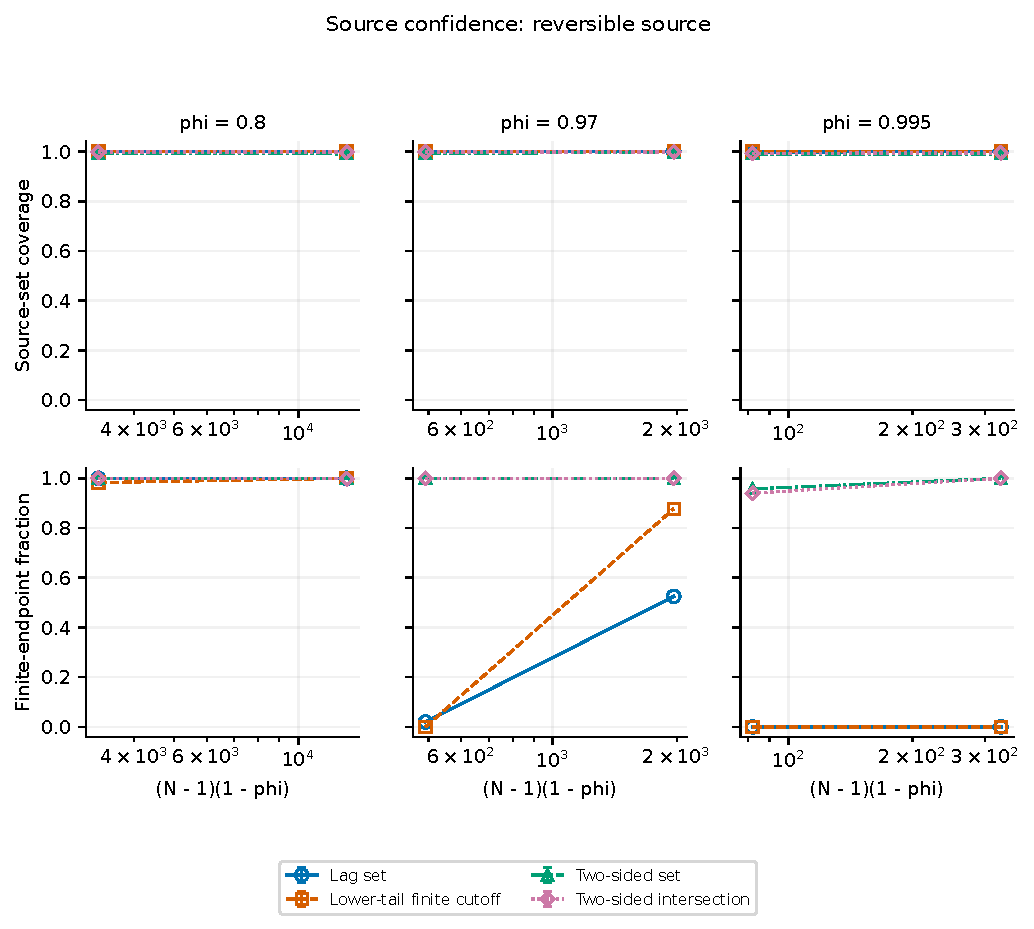
\includegraphics[width=7in]{figures/source_confidence_null.pdf}}
\caption{Coverage and finite endpoints differ across source constructions. Core null cells have 400 records, except $\phi=0.97,N=65537$, which has 1000. Coverage bars are pointwise 95\% binomial intervals. All fractions use the complete cell. The source confidence error is $0.005$, distinct from the display interval. Coincident curves have equal fractions; methods remain in the legend. Values are saved study results.}\label{fig:study16-source-null}
\end{figure}

\begin{figure}[p]
\centering
\makebox[\textwidth][c]{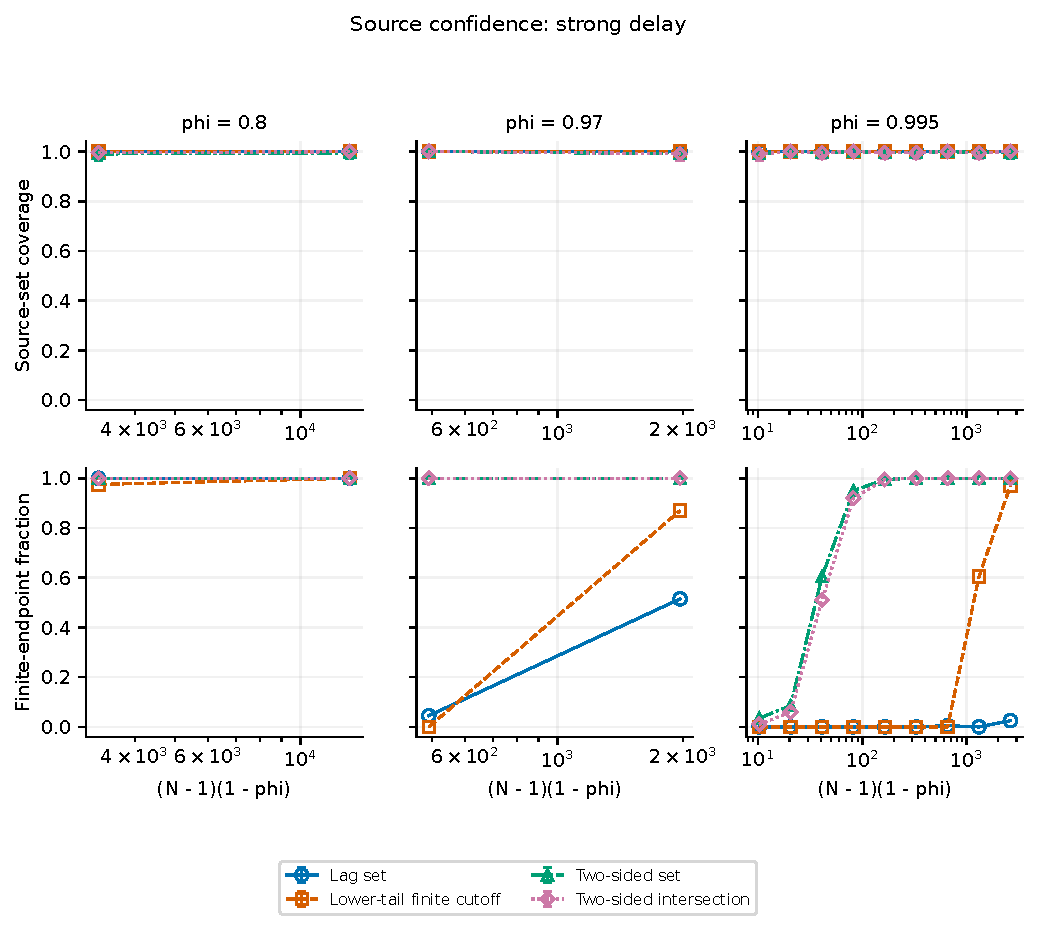
\includegraphics[width=7in]{figures/source_confidence_strong.pdf}}
\caption{Strong-delay records can have covered source sets without finite upper endpoints. Each condition has 200 records. The display includes the nine-length $\phi=0.995$ curve and both core lengths at other persistences. Coverage bars are pointwise 95\% binomial intervals; endpoint fractions use all records. Equal curves indicate equal fractions. The source-set error allowance is $0.005$. Values are saved study results.}\label{fig:study16-source-strong}
\end{figure}

\begin{figure}[p]
\centering
\makebox[\textwidth][c]{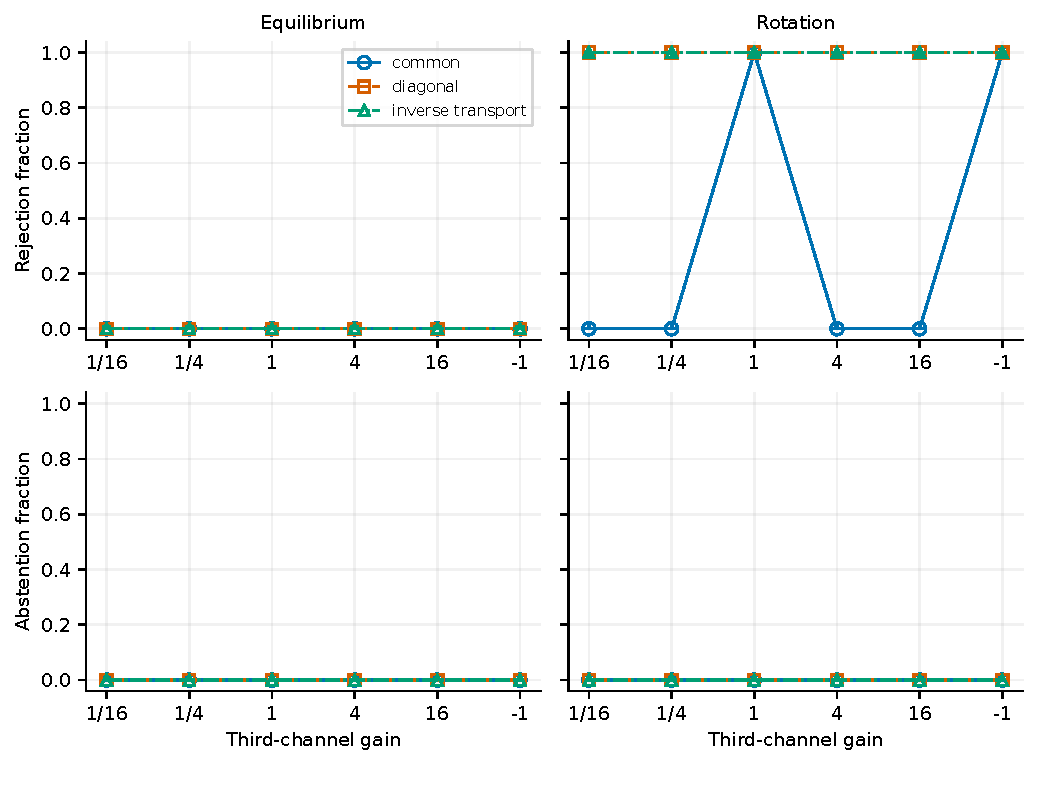
\includegraphics[width=7in]{figures/gain_controls.pdf}}
\caption{Diagonal bounds and inverse transport preserve all rotating-source rejections across six gains. The common scalar rule loses every rejection at four gains. Null and rotating cells have 400 and 200 records, respectively, with methods paired on each record. All abstention fractions and equilibrium rejection fractions are zero. These transformations change data and bounds together. Values are saved study results.}\label{fig:study16-gains}
\end{figure}

\begin{figure}[p]
\centering
\makebox[\textwidth][c]{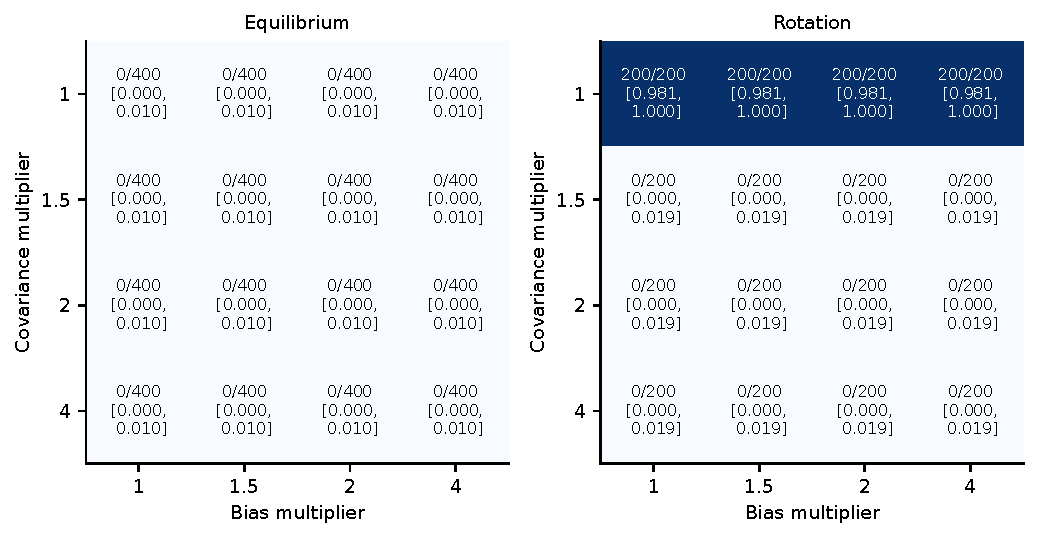
\includegraphics[width=7in]{figures/bound_inflation.pdf}}
\caption{Conservative covariance inflation removes rotating-source rejections within this grid. All 16 covariance/bias factor pairs are shown for both regimes, with 400 null or 200 rotating records. Entries give rejection counts and pointwise 95\% binomial intervals, rounded outward to $0.001$. No cell has an abstention. Equal counts across bias factors do not establish equal thresholds. Values are saved study results.}\label{fig:study16-inflation}
\end{figure}
